% Created by tikzDevice version 0.8.1 on 2015-11-17 12:15:23
% !TEX encoding = UTF-8 Unicode
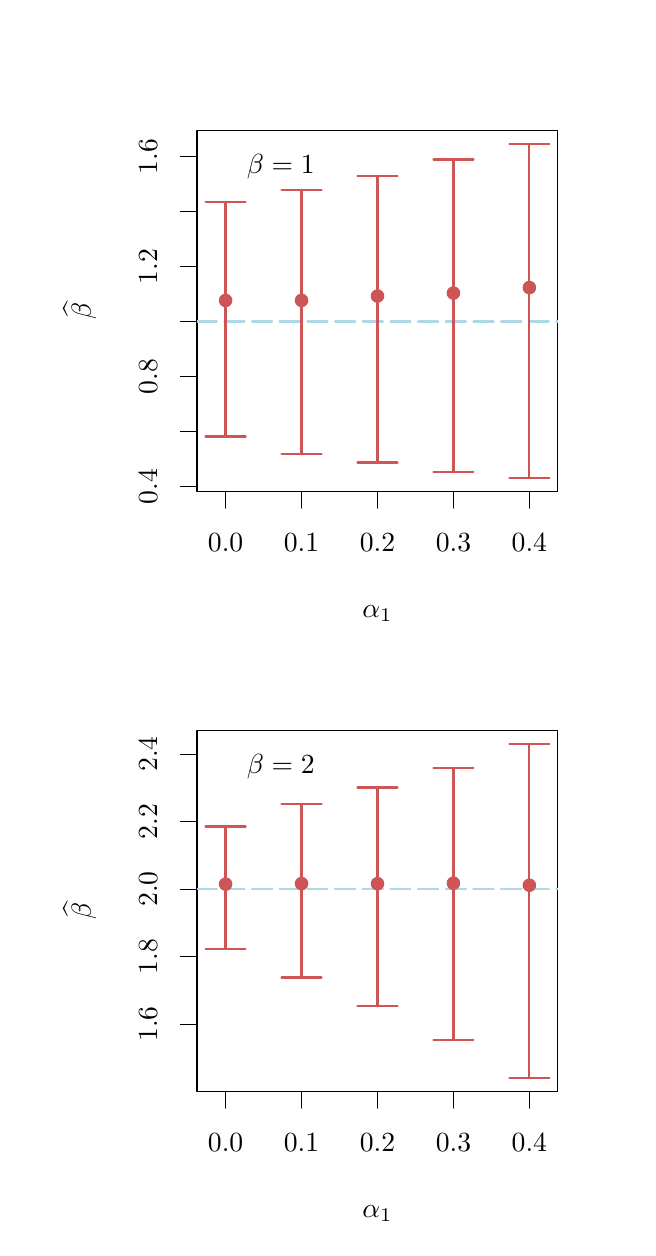
\begin{tikzpicture}[x=1pt,y=1pt]
\definecolor{fillColor}{RGB}{255,255,255}
\path[use as bounding box,fill=fillColor,fill opacity=0.00] (0,0) rectangle (216.81,433.62);
\begin{scope}
\path[clip] ( 61.20,266.01) rectangle (191.61,396.42);
\definecolor{drawColor}{RGB}{255,255,255}
\definecolor{fillColor}{RGB}{255,255,255}

\path[draw=drawColor,line width= 0.4pt,line join=round,line cap=round,fill=fillColor] ( 71.52,335.05) circle (  2.25);

\path[draw=drawColor,line width= 0.4pt,line join=round,line cap=round,fill=fillColor] ( 98.96,335.07) circle (  2.25);

\path[draw=drawColor,line width= 0.4pt,line join=round,line cap=round,fill=fillColor] (126.41,336.65) circle (  2.25);

\path[draw=drawColor,line width= 0.4pt,line join=round,line cap=round,fill=fillColor] (153.85,337.71) circle (  2.25);

\path[draw=drawColor,line width= 0.4pt,line join=round,line cap=round,fill=fillColor] (181.29,339.70) circle (  2.25);
\end{scope}
\begin{scope}
\path[clip] (  0.00,  0.00) rectangle (216.81,433.62);
\definecolor{drawColor}{RGB}{0,0,0}

\path[draw=drawColor,line width= 0.4pt,line join=round,line cap=round] ( 71.52,266.01) -- (181.29,266.01);

\path[draw=drawColor,line width= 0.4pt,line join=round,line cap=round] ( 71.52,266.01) -- ( 71.52,260.01);

\path[draw=drawColor,line width= 0.4pt,line join=round,line cap=round] ( 98.96,266.01) -- ( 98.96,260.01);

\path[draw=drawColor,line width= 0.4pt,line join=round,line cap=round] (126.41,266.01) -- (126.41,260.01);

\path[draw=drawColor,line width= 0.4pt,line join=round,line cap=round] (153.85,266.01) -- (153.85,260.01);

\path[draw=drawColor,line width= 0.4pt,line join=round,line cap=round] (181.29,266.01) -- (181.29,260.01);

\node[text=drawColor,anchor=base,inner sep=0pt, outer sep=0pt, scale=  1.00] at ( 71.52,244.41) {0.0};

\node[text=drawColor,anchor=base,inner sep=0pt, outer sep=0pt, scale=  1.00] at ( 98.96,244.41) {0.1};

\node[text=drawColor,anchor=base,inner sep=0pt, outer sep=0pt, scale=  1.00] at (126.41,244.41) {0.2};

\node[text=drawColor,anchor=base,inner sep=0pt, outer sep=0pt, scale=  1.00] at (153.85,244.41) {0.3};

\node[text=drawColor,anchor=base,inner sep=0pt, outer sep=0pt, scale=  1.00] at (181.29,244.41) {0.4};

\path[draw=drawColor,line width= 0.4pt,line join=round,line cap=round] ( 61.20,267.81) -- ( 61.20,387.00);

\path[draw=drawColor,line width= 0.4pt,line join=round,line cap=round] ( 61.20,267.81) -- ( 55.20,267.81);

\path[draw=drawColor,line width= 0.4pt,line join=round,line cap=round] ( 61.20,287.68) -- ( 55.20,287.68);

\path[draw=drawColor,line width= 0.4pt,line join=round,line cap=round] ( 61.20,307.54) -- ( 55.20,307.54);

\path[draw=drawColor,line width= 0.4pt,line join=round,line cap=round] ( 61.20,327.41) -- ( 55.20,327.41);

\path[draw=drawColor,line width= 0.4pt,line join=round,line cap=round] ( 61.20,347.27) -- ( 55.20,347.27);

\path[draw=drawColor,line width= 0.4pt,line join=round,line cap=round] ( 61.20,367.14) -- ( 55.20,367.14);

\path[draw=drawColor,line width= 0.4pt,line join=round,line cap=round] ( 61.20,387.00) -- ( 55.20,387.00);

\node[text=drawColor,rotate= 90.00,anchor=base,inner sep=0pt, outer sep=0pt, scale=  1.00] at ( 46.80,267.81) {0.4};

\node[text=drawColor,rotate= 90.00,anchor=base,inner sep=0pt, outer sep=0pt, scale=  1.00] at ( 46.80,307.54) {0.8};

\node[text=drawColor,rotate= 90.00,anchor=base,inner sep=0pt, outer sep=0pt, scale=  1.00] at ( 46.80,347.27) {1.2};

\node[text=drawColor,rotate= 90.00,anchor=base,inner sep=0pt, outer sep=0pt, scale=  1.00] at ( 46.80,387.00) {1.6};

\path[draw=drawColor,line width= 0.4pt,line join=round,line cap=round] ( 61.20,266.01) --
	(191.61,266.01) --
	(191.61,396.42) --
	( 61.20,396.42) --
	( 61.20,266.01);
\end{scope}
\begin{scope}
\path[clip] (  0.00,216.81) rectangle (216.81,433.62);
\definecolor{drawColor}{RGB}{0,0,0}

\node[text=drawColor,anchor=base,inner sep=0pt, outer sep=0pt, scale=  1.00] at (126.41,220.41) {$\alpha_1$};

\node[text=drawColor,rotate= 90.00,anchor=base,inner sep=0pt, outer sep=0pt, scale=  1.00] at ( 22.80,331.22) {$\widehat{\beta}$};
\end{scope}
\begin{scope}
\path[clip] ( 61.20,266.01) rectangle (191.61,396.42);
\definecolor{drawColor}{RGB}{0,0,0}

\node[text=drawColor,anchor=base west,inner sep=0pt, outer sep=0pt, scale=  1.00] at ( 79.20,380.98) {$\beta=1$};
\definecolor{drawColor}{RGB}{173,216,230}

\path[draw=drawColor,line width= 0.8pt,dash pattern=on 7pt off 3pt ,line join=round,line cap=round] ( 61.20,327.41) -- (191.61,327.41);

\path[draw=drawColor,line width= 0.8pt,dash pattern=on 7pt off 3pt ,line join=round,line cap=round] ( 61.20,327.41) -- (191.61,327.41);

\path[draw=drawColor,line width= 0.8pt,dash pattern=on 7pt off 3pt ,line join=round,line cap=round] ( 61.20,327.41) -- (191.61,327.41);

\path[draw=drawColor,line width= 0.8pt,dash pattern=on 7pt off 3pt ,line join=round,line cap=round] ( 61.20,327.41) -- (191.61,327.41);

\path[draw=drawColor,line width= 0.8pt,dash pattern=on 7pt off 3pt ,line join=round,line cap=round] ( 61.20,327.41) -- (191.61,327.41);
\definecolor{drawColor}{RGB}{205,85,85}

\path[draw=drawColor,line width= 0.8pt,line join=round,line cap=round] ( 71.52,285.87) -- ( 71.52,370.49);

\path[draw=drawColor,line width= 0.8pt,line join=round,line cap=round] ( 64.29,285.87) --
	( 71.52,285.87) --
	( 78.75,285.87);

\path[draw=drawColor,line width= 0.8pt,line join=round,line cap=round] ( 78.75,370.49) --
	( 71.52,370.49) --
	( 64.29,370.49);

\path[draw=drawColor,line width= 0.8pt,line join=round,line cap=round] ( 98.96,279.52) -- ( 98.96,375.05);

\path[draw=drawColor,line width= 0.8pt,line join=round,line cap=round] ( 91.73,279.52) --
	( 98.96,279.52) --
	(106.19,279.52);

\path[draw=drawColor,line width= 0.8pt,line join=round,line cap=round] (106.19,375.05) --
	( 98.96,375.05) --
	( 91.73,375.05);

\path[draw=drawColor,line width= 0.8pt,line join=round,line cap=round] (126.41,276.52) -- (126.41,380.04);

\path[draw=drawColor,line width= 0.8pt,line join=round,line cap=round] (119.18,276.52) --
	(126.41,276.52) --
	(133.63,276.52);

\path[draw=drawColor,line width= 0.8pt,line join=round,line cap=round] (133.63,380.04) --
	(126.41,380.04) --
	(119.18,380.04);

\path[draw=drawColor,line width= 0.8pt,line join=round,line cap=round] (153.85,272.99) -- (153.85,386.00);

\path[draw=drawColor,line width= 0.8pt,line join=round,line cap=round] (146.62,272.99) --
	(153.85,272.99) --
	(161.08,272.99);

\path[draw=drawColor,line width= 0.8pt,line join=round,line cap=round] (161.08,386.00) --
	(153.85,386.00) --
	(146.62,386.00);

\path[draw=drawColor,line width= 0.8pt,line join=round,line cap=round] (181.29,270.84) -- (181.29,391.59);

\path[draw=drawColor,line width= 0.8pt,line join=round,line cap=round] (174.06,270.84) --
	(181.29,270.84) --
	(188.52,270.84);

\path[draw=drawColor,line width= 0.8pt,line join=round,line cap=round] (188.52,391.59) --
	(181.29,391.59) --
	(174.06,391.59);
\definecolor{fillColor}{RGB}{205,85,85}

\path[draw=drawColor,line width= 0.4pt,line join=round,line cap=round,fill=fillColor] ( 71.52,335.05) circle (  2.25);

\path[draw=drawColor,line width= 0.4pt,line join=round,line cap=round,fill=fillColor] ( 98.96,335.07) circle (  2.25);

\path[draw=drawColor,line width= 0.4pt,line join=round,line cap=round,fill=fillColor] (126.41,336.65) circle (  2.25);

\path[draw=drawColor,line width= 0.4pt,line join=round,line cap=round,fill=fillColor] (153.85,337.71) circle (  2.25);

\path[draw=drawColor,line width= 0.4pt,line join=round,line cap=round,fill=fillColor] (181.29,339.70) circle (  2.25);
\end{scope}
\begin{scope}
\path[clip] ( 61.20, 49.20) rectangle (191.61,179.61);
\definecolor{drawColor}{RGB}{255,255,255}
\definecolor{fillColor}{RGB}{255,255,255}

\path[draw=drawColor,line width= 0.4pt,line join=round,line cap=round,fill=fillColor] ( 71.52,124.14) circle (  2.25);

\path[draw=drawColor,line width= 0.4pt,line join=round,line cap=round,fill=fillColor] ( 98.96,124.33) circle (  2.25);

\path[draw=drawColor,line width= 0.4pt,line join=round,line cap=round,fill=fillColor] (126.41,124.30) circle (  2.25);

\path[draw=drawColor,line width= 0.4pt,line join=round,line cap=round,fill=fillColor] (153.85,124.47) circle (  2.25);

\path[draw=drawColor,line width= 0.4pt,line join=round,line cap=round,fill=fillColor] (181.29,123.74) circle (  2.25);
\end{scope}
\begin{scope}
\path[clip] (  0.00,  0.00) rectangle (216.81,433.62);
\definecolor{drawColor}{RGB}{0,0,0}

\path[draw=drawColor,line width= 0.4pt,line join=round,line cap=round] ( 71.52, 49.20) -- (181.29, 49.20);

\path[draw=drawColor,line width= 0.4pt,line join=round,line cap=round] ( 71.52, 49.20) -- ( 71.52, 43.20);

\path[draw=drawColor,line width= 0.4pt,line join=round,line cap=round] ( 98.96, 49.20) -- ( 98.96, 43.20);

\path[draw=drawColor,line width= 0.4pt,line join=round,line cap=round] (126.41, 49.20) -- (126.41, 43.20);

\path[draw=drawColor,line width= 0.4pt,line join=round,line cap=round] (153.85, 49.20) -- (153.85, 43.20);

\path[draw=drawColor,line width= 0.4pt,line join=round,line cap=round] (181.29, 49.20) -- (181.29, 43.20);

\node[text=drawColor,anchor=base,inner sep=0pt, outer sep=0pt, scale=  1.00] at ( 71.52, 27.60) {0.0};

\node[text=drawColor,anchor=base,inner sep=0pt, outer sep=0pt, scale=  1.00] at ( 98.96, 27.60) {0.1};

\node[text=drawColor,anchor=base,inner sep=0pt, outer sep=0pt, scale=  1.00] at (126.41, 27.60) {0.2};

\node[text=drawColor,anchor=base,inner sep=0pt, outer sep=0pt, scale=  1.00] at (153.85, 27.60) {0.3};

\node[text=drawColor,anchor=base,inner sep=0pt, outer sep=0pt, scale=  1.00] at (181.29, 27.60) {0.4};

\path[draw=drawColor,line width= 0.4pt,line join=round,line cap=round] ( 61.20, 73.55) -- ( 61.20,171.13);

\path[draw=drawColor,line width= 0.4pt,line join=round,line cap=round] ( 61.20, 73.55) -- ( 55.20, 73.55);

\path[draw=drawColor,line width= 0.4pt,line join=round,line cap=round] ( 61.20, 97.95) -- ( 55.20, 97.95);

\path[draw=drawColor,line width= 0.4pt,line join=round,line cap=round] ( 61.20,122.34) -- ( 55.20,122.34);

\path[draw=drawColor,line width= 0.4pt,line join=round,line cap=round] ( 61.20,146.73) -- ( 55.20,146.73);

\path[draw=drawColor,line width= 0.4pt,line join=round,line cap=round] ( 61.20,171.13) -- ( 55.20,171.13);

\node[text=drawColor,rotate= 90.00,anchor=base,inner sep=0pt, outer sep=0pt, scale=  1.00] at ( 46.80, 73.55) {1.6};

\node[text=drawColor,rotate= 90.00,anchor=base,inner sep=0pt, outer sep=0pt, scale=  1.00] at ( 46.80, 97.95) {1.8};

\node[text=drawColor,rotate= 90.00,anchor=base,inner sep=0pt, outer sep=0pt, scale=  1.00] at ( 46.80,122.34) {2.0};

\node[text=drawColor,rotate= 90.00,anchor=base,inner sep=0pt, outer sep=0pt, scale=  1.00] at ( 46.80,146.73) {2.2};

\node[text=drawColor,rotate= 90.00,anchor=base,inner sep=0pt, outer sep=0pt, scale=  1.00] at ( 46.80,171.13) {2.4};

\path[draw=drawColor,line width= 0.4pt,line join=round,line cap=round] ( 61.20, 49.20) --
	(191.61, 49.20) --
	(191.61,179.61) --
	( 61.20,179.61) --
	( 61.20, 49.20);
\end{scope}
\begin{scope}
\path[clip] (  0.00,  0.00) rectangle (216.81,216.81);
\definecolor{drawColor}{RGB}{0,0,0}

\node[text=drawColor,anchor=base,inner sep=0pt, outer sep=0pt, scale=  1.00] at (126.41,  3.60) {$\alpha_1$};

\node[text=drawColor,rotate= 90.00,anchor=base,inner sep=0pt, outer sep=0pt, scale=  1.00] at ( 22.80,114.41) {$\widehat{\beta}$};
\end{scope}
\begin{scope}
\path[clip] ( 61.20, 49.20) rectangle (191.61,179.61);
\definecolor{drawColor}{RGB}{0,0,0}

\node[text=drawColor,anchor=base west,inner sep=0pt, outer sep=0pt, scale=  1.00] at ( 79.20,164.17) {$\beta=2$};
\definecolor{drawColor}{RGB}{173,216,230}

\path[draw=drawColor,line width= 0.8pt,dash pattern=on 7pt off 3pt ,line join=round,line cap=round] ( 61.20,122.34) -- (191.61,122.34);

\path[draw=drawColor,line width= 0.8pt,dash pattern=on 7pt off 3pt ,line join=round,line cap=round] ( 61.20,122.34) -- (191.61,122.34);

\path[draw=drawColor,line width= 0.8pt,dash pattern=on 7pt off 3pt ,line join=round,line cap=round] ( 61.20,122.34) -- (191.61,122.34);

\path[draw=drawColor,line width= 0.8pt,dash pattern=on 7pt off 3pt ,line join=round,line cap=round] ( 61.20,122.34) -- (191.61,122.34);

\path[draw=drawColor,line width= 0.8pt,dash pattern=on 7pt off 3pt ,line join=round,line cap=round] ( 61.20,122.34) -- (191.61,122.34);
\definecolor{drawColor}{RGB}{205,85,85}

\path[draw=drawColor,line width= 0.8pt,line join=round,line cap=round] ( 71.52,100.80) -- ( 71.52,144.93);

\path[draw=drawColor,line width= 0.8pt,line join=round,line cap=round] ( 64.29,100.80) --
	( 71.52,100.80) --
	( 78.75,100.80);

\path[draw=drawColor,line width= 0.8pt,line join=round,line cap=round] ( 78.75,144.93) --
	( 71.52,144.93) --
	( 64.29,144.93);

\path[draw=drawColor,line width= 0.8pt,line join=round,line cap=round] ( 98.96, 90.36) -- ( 98.96,153.00);

\path[draw=drawColor,line width= 0.8pt,line join=round,line cap=round] ( 91.73, 90.36) --
	( 98.96, 90.36) --
	(106.19, 90.36);

\path[draw=drawColor,line width= 0.8pt,line join=round,line cap=round] (106.19,153.00) --
	( 98.96,153.00) --
	( 91.73,153.00);

\path[draw=drawColor,line width= 0.8pt,line join=round,line cap=round] (126.41, 80.02) -- (126.41,159.09);

\path[draw=drawColor,line width= 0.8pt,line join=round,line cap=round] (119.18, 80.02) --
	(126.41, 80.02) --
	(133.63, 80.02);

\path[draw=drawColor,line width= 0.8pt,line join=round,line cap=round] (133.63,159.09) --
	(126.41,159.09) --
	(119.18,159.09);

\path[draw=drawColor,line width= 0.8pt,line join=round,line cap=round] (153.85, 67.78) -- (153.85,166.05);

\path[draw=drawColor,line width= 0.8pt,line join=round,line cap=round] (146.62, 67.78) --
	(153.85, 67.78) --
	(161.08, 67.78);

\path[draw=drawColor,line width= 0.8pt,line join=round,line cap=round] (161.08,166.05) --
	(153.85,166.05) --
	(146.62,166.05);

\path[draw=drawColor,line width= 0.8pt,line join=round,line cap=round] (181.29, 54.03) -- (181.29,174.78);

\path[draw=drawColor,line width= 0.8pt,line join=round,line cap=round] (174.06, 54.03) --
	(181.29, 54.03) --
	(188.52, 54.03);

\path[draw=drawColor,line width= 0.8pt,line join=round,line cap=round] (188.52,174.78) --
	(181.29,174.78) --
	(174.06,174.78);
\definecolor{fillColor}{RGB}{205,85,85}

\path[draw=drawColor,line width= 0.4pt,line join=round,line cap=round,fill=fillColor] ( 71.52,124.14) circle (  2.25);

\path[draw=drawColor,line width= 0.4pt,line join=round,line cap=round,fill=fillColor] ( 98.96,124.33) circle (  2.25);

\path[draw=drawColor,line width= 0.4pt,line join=round,line cap=round,fill=fillColor] (126.41,124.30) circle (  2.25);

\path[draw=drawColor,line width= 0.4pt,line join=round,line cap=round,fill=fillColor] (153.85,124.47) circle (  2.25);

\path[draw=drawColor,line width= 0.4pt,line join=round,line cap=round,fill=fillColor] (181.29,123.74) circle (  2.25);
\end{scope}
\end{tikzpicture}
